\chapter{Neuromuscular Model}\label{sec:neuro_model}
\begin{marginfigure}
    \centering
    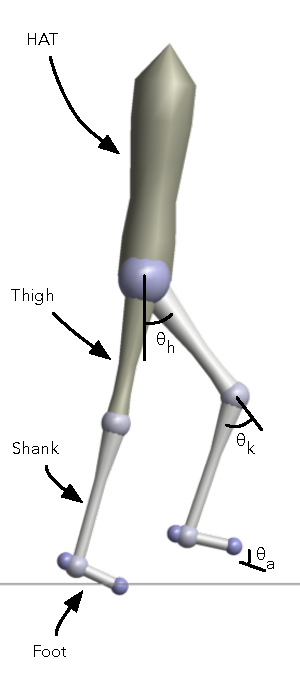
\includegraphics[width=\linewidth]{neuro_mech_model}
    \caption{The skeletal model we use to simulate neuromuscular reflex control.
    The model consists of seven segments: left and right feet, shanks, and
    thighs, as well as a lumped head-arms-trunk (HAT) segment. Flexion joint
    angles are positive, extension joint angles are negative, and the zero
    angle configuration represents standing.}
    \label{fig:neuro_seven_link}
\end{marginfigure}

In this thesis we intend to investigate the ability of neuromuscular reflex
control to improve amputee gait robustness. To this end, here we provide a more
detailed review the neuromuscular model components on which we base our
prosthesis control. Four parts comprise the model: a mechanical simulation
environment we use to obtain simulation results (\cref{sec:neuro_mech_model}),
biological motors modeled by the hill muscle model that apply torques to joints
(\cref{sec:neuro_hill_muscle}), and finally functionally-motivated stance
(\cref{sec:neuro_stance_reflexes}) and swing (\cref{sec:neuro_swing_reflexes})
reflexes that implement the key behaviors required for walking.

\section{Mechanical Model}\label{sec:neuro_mech_model}

To obtain the simulation results we present in \cref{sec:completed_comparison},
we construct a mechanical model in the Matlab Simscape Multibody environment
similar to those presented in \citet{geyer2010muscle, song2013integration,
song2015neural}.  This model represents the seven link biped in
\cref{fig:neuro_seven_link} and includes two legs with thigh, shank, and foot
segments as well as a lumped head-arms-trunk (HAT) segment.
\Cref{tab:model_mech_params} lists the segment lengths, center of mass and joint
locations measured from the distal end, masses, and inertias that approximate
those of a \unit[80]{kg}, \unit[2.0]{m} tall person.

\begin{table}[b]
  \centering
      \begin{tabular}{lllll}
        \toprule
        & Feet & Shanks & Thighs & HAT \\
        \midrule
        $l         \ (\unit{cm})$ & 20    & 50   & 50   & 80   \\
        $d_\tn{COM}   \ (\unit{cm})$ & 14    & 30   & 30   & 35   \\
        $d_\tn{Joint} \ (\unit{cm})$ & 16    & 50   & 50   &      \\
        $m         \ (\unit{kg})$ & 1.25  & 3.5  & 8.5  & 53.5 \\
        $J         \ (\unit{kg})$ & 0.005 & 0.05 & 0.15 & 3    \\
        \bottomrule
      \end{tabular}
  \caption{Segment lengths $(l_s)$, center of mass $(d_\tn{COM})$ and joint
  $(d_\tn{Joint})$ locations measured from the distal end, masses $(m)$, and
  inertias $(J)$ approximated from
  \citet{gunther2003synthesis}.}\label{tab:model_mech_params}
\end{table}

The mechanical model interacts with the environment through ground reaction
forces on the toes and balls of the feet. Specifically, we use a 2-dimensional
reduction of the 3D ground contact model presented in
\citet{song2013generalization} to calculate forces in the normal and
tangential directions with respect to the terrain. In the normal direction the
force is
\begin{align}
    F_\tn{n} = k_\tn{n} \Delta n_c (1 + \dot n_c) (\Delta n_c > 0)
    \left(\nicefrac{\dot n_c}{v_\tn{max}} > -1 \right),
    \label{eq:grf_n}
\end{align}
where $k_\tn{n} = \unitfrac[78.45]{N}{mm}$ is the stiffness coefficient in
the normal direction and $\Delta n_c$ and $\dot n_c$ are the normal penetration
in the normal direction and velocity. The form of the normal force is inspired
by \citet{gunther2003synthesis, scott1993biomechanical} and represents a linear
spring with multiplicitive damping.  $v_\tn{max} = \unitfrac[3]{cm}{s}$ represents
the maximum recovery velocity of the ground. If $\dot n_c$ exceeds this
velocity ground contact is lost.

In the tangential direction, a state machine switches between two force models
representing sliding and static friction. Sliding friction is given by
\begin{align}
    F_{\tn{t,slide}} = -\func{sign}{\dot t_c} \mu_\tn{slide} F_n
\end{align}
while static friction is given by
\begin{align}
    F_{\tn{t,static}} = -k_t \Delta t_c \left(1 + \func{sign}{\Delta t_c}
    \frac{\dot t_c}{v_\tn{max}} \right),
\end{align}
where $\Delta t_c$ is the penetration in the tangential direction $\dot t_c$ is
the penetration velocity, $\mu_\tn{slide} = 0.8$ is the sliding coefficient of
friction, and $k_\tn{t} =\unitfrac[78.45]{N}{mm}$ is the stiffness coefficient
in the tangential direction.

The contact model begins in the sliding mode and switches to the static mode if
$\dot t_c < 1 \unitfrac[1]{cm}{s}$. It switches back to the sliding mode when $|
F_{\tn{t,static}} | < \mu_\tn{static} | F_n |$, where $\mu_\tn{static} = 0.9$.

Finally, the biped skeletal model includes soft joint limits to represent
the skeletal joint limits on the knee, ankle, and hip joints. The functional
form form the soft limit joint torque is identical to that of the normal ground
reaction force given by \cref{eq:grf_n}.
\begin{align}
    \tau_{jl} = k_{jl} \Delta \phi_{jl} (1 + \dot \phi_{jl}) (\Delta
    \phi_{jl}  > 0) \left(\nicefrac{\dot \phi_{jl}}{\dot \phi_\tn{max}} > -1
    \right), 
    \label{eq:tau_joint_limit}
\end{align}
where $k_{jl} = \unitfrac[0.3]{N \cdot m}{deg}$ is the joint stiffness $\Delta
\phi$ and $\dot \phi_{jl}$ are the joint limit penetration angle and
velocity respectively, and $\dot \phi_\tn{max} = \unitfrac[1]{deg}{s}$ is the
maximum joint limit retraction velocity. \Cref{tab:joint_lim} lists the
engagement angles for the joint limits.
\begin{margintable}[-0.65in]
  \centering
      \begin{tabular}{lll}
        \toprule
        Joint & ext.\ lim.\ & flex lim.\ \\
        \midrule
        hip   &     & 50 \\
        knee  &   5 &    \\
        ankle & -40 & 20 \\
        \bottomrule
      \end{tabular}
  \caption{Joint limits for the hip, knee, and ankle joints listed in degrees.
  Positive joint angles represent flexion and negative joint angles represent
  extension (see \cref{fig:neuro_seven_link}).}\label{tab:joint_lim}
\end{margintable}

To obtain simulation results, we simulate the mechanical system with the ode15s
variable step solver. We set the maximum step size to \unit[10]{ms}, relative
error tolerance to $10^{-4}$, and abolute error to $10^{-6}$.

\section{Hill Muscle Models}\label{sec:neuro_hill_muscle}
\begin{marginfigure}[-0.25in]
    \centering
    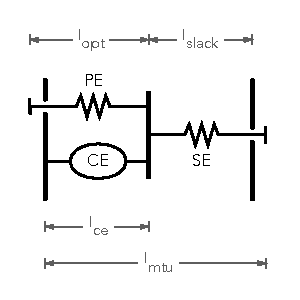
\includegraphics[width=\linewidth]{mtu_figure}
    \vspace{-0.4in}
    \caption{Hill-type muscle tendon unit with contractile element (CE),
    parallel elasticity (PE), and series elasticity (SE).}
    \label{fig:hill_type_mtu}
\end{marginfigure}
Our proposed transfemoral prosthesis control is comprised of biological muscle
actuators that are stimulated according to hypothesized reflex pathways.
Specifically, we use a Hill-type \emph{muscle tendon unit} (MTU) developed in
\citet{geyer2010muscle}. It is comprised of a contractile element (CE) that
represents muscle fibers and produces force when activated, a parallel elastic
(PE) element that represents the stiffness of the collagen tissue between muscle
fascicles, and series elastic (SE) element that models tendon stretch.
\Cref{fig:hill_type_mtu} shows the arrangement of these elements. Note that the
PE and SE both are unidirectional springs with engagement lengths of
$l_\tn{opt}$ and $l_\tn{slack}$ respectively.

The CE generates force according to
\begin{align}
    F_\tn{CE} = F_\tn{max} A \func{f_l}{l_\tn{CE}} \func{f_v}{v_\tn{CE}}.
    \label{eq:hill_ce}
\end{align}
In this equation, the force generated by the CE $(F_\tn{CE})$ is the maximum
isometric (constant length) force $(F_\tn{max})$ multiplied by activation $(A)$,
the force-length ($\func{f_l}{\cdot})$, and force-velocity
$(\func{f_v}{\cdot})$, relationships of the CE. The activation $A$ is a low-pass
filtered version of the stimulation signal muscle $S(t)$ generated by the muscle
reflexes we will detail in the \hyperref[sec:neuro_stance_reflexes]{next}
section. This filter, given by $A(t) = S - \tau \dot A(t)$ with time constant
$\tau$, represents the diffusion dynamics of calcium ions that activate binding
sites in the muscle fibers.
\begin{marginfigure}[-1in]
    \centering
    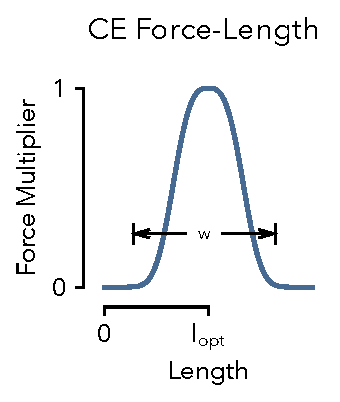
\includegraphics[width=\linewidth]{force_length_ce_annotate}
    \vspace{-0.25in}
    \caption{Force-length relationship of the CE.}
    \label{fig:force_length_ce}
\end{marginfigure}

The binding sites are where overlapping actin and myosin filaments attach and
generate pulling force. The contractile element length of $l_\tn{opt}$
corresponds to maximum overlap between these filaments. Therefore, as as the
muscle length moves away from $l_\tn{opt}$, its force production capacity
decreases leading to the force-length relationship shown in
\cref{fig:force_length_ce}. We model the force-length relationship via a bell
curve
\begin{align}
    \func{f_l}{l_\tn{CE}} = \exp \left( \ln(0.05) \left|
    \frac{l_\tn{CE} - l_\tn{opt}}{w l_\tn{opt}}
    \right|^3 \right).
    \label{eq:hill_force_length}
\end{align}
\begin{marginfigure}[0.25in]
    \centering
    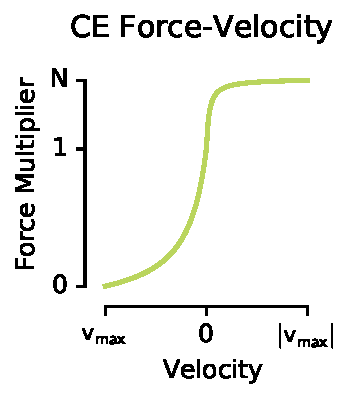
\includegraphics[width=\linewidth]{force_velocity_ce}
    \vspace{-0.25in}
    \caption{Force-velocity relationship of the CE.}
    \label{fig:force_velocity_ce}
\end{marginfigure}

The velocity-dependent filament attachment probabilities give rise to a
force-velocity relationship shown in \cref{fig:force_velocity_ce}. The following
expression captures this relationship.
\begin{table}[t]
  \centering
  \begin{tabular}{ll|ll}
    \toprule
    Param & Value             & Param                   & Value \\
    \midrule                           
    $\tau$ & \unit[0.1]{s}    & $l_\tn{opt}^\tn{ham}$   & \unit[0.10]{m} \\
    $w$    & 0.56             & $v_\tn{max}^\tn{ham}$   & \unitfrac[-1.2]{m}{s} \\
    $K$    & 5                & $F_\tn{max}^\tn{ham}$   & \unit[3000]{N} \\
    $N$    & 1.5              & $l_\tn{slack}^\tn{ham}$ & \unit[0.31]{m} \\
    $\epsilon_\tn{PE}$ & $w$  &                         & \\
    $\epsilon_\tn{SE}$ & 0.04 &                         & \\
    \bottomrule
  \end{tabular}
  \caption{Neuromuscular parameters for shared entities (left) and the hamstring
  muscle (right)}
  \label{tab:neuromusc_params}
\end{table}
\begin{align}
    \func{f_v}{v_\tn{CE}} = 
    \begin{cases} 
        \frac{v_\tn{max} - v_\tn{CE}}{v_\tn{max} + K v_\tn{CE}}, & \tn{if } v_\tn{CE}< 0 \\
        N + (N-1) \frac{v_\tn{max} + v_\tn{CE}}{7.56 K v_\tn{CE} - v_\tn{max}}, &
            \tn{if } v_\tn{CE} \ge 0 
    \end{cases}
\end{align}
In this expression, $K$ is a shape parameter and $N$ determines the force
amplification when the contractile element is lengthening. The force-velocity
relationship acts as a multiplicative damper causing the CE to produce more
contractile force when it is lengthening and less as it extends.

We model both passive elements, the PE and SE, using the same functional form
representing a unidirectional, stiffening spring, the behavior of which is shown
in \cref{fig:force_length_pese}. The expressions for the elastic force produces
by these elements are
\begin{align}
    \func{F_\tn{PE}}{l_\tn{CE}} &= F_\tn{max} \left( \frac{l_\tn{CE} - l_\tn{opt}}{\epsilon_\tn{PE}
        l_\tn{opt}} \right)^2 (l_\tn{CE} > l_\tn{opt})\\
    \func{F_\tn{SE}}{l_\tn{SE}} &= F_\tn{max} \left( \frac{l_\tn{SE} - l_\tn{slack}}{\epsilon_\tn{SE}
        l_\tn{slack}} \right)^2 (l_\tn{SE} > l_\tn{slack}).
\end{align}
\begin{marginfigure}
    \centering
    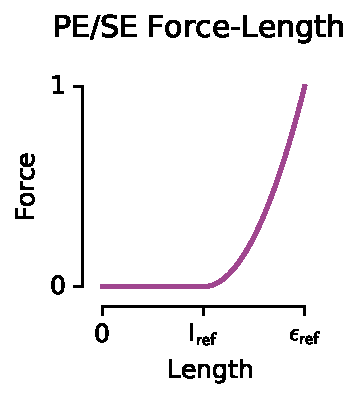
\includegraphics[width=\linewidth]{force_length_pese}
    \caption{PE and SE force length relationship. For the PE, $l_\tn{ref} = l_\tn{opt}$
    and $\epsilon_\tn{ref} = \epsilon_\tn{PE}$. Likewise, for the SE, $l_\tn{ref} =
    l_\tn{slack}$ and $\epsilon_\tn{ref} = \epsilon_\tn{SE}$.} 
    \label{fig:force_length_pese}
\end{marginfigure}

The left-hand side of \cref{tab:neuromusc_params} lists the parameters common
among all seven muscles of each leg of the neuromuscular model. On the
right-hand side of the table, we list four muscle-specific parameters for
hamstrings muscle. For a complete list of muscle parameters please refer
to \citet{song2015neural}. 

\begin{figure}[b]
    \centering
    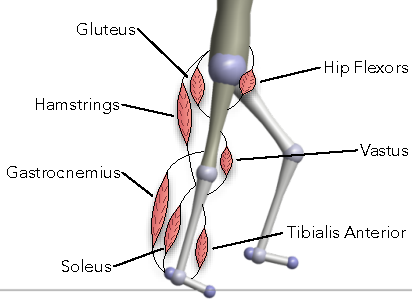
\includegraphics[width=3in]{biped_w_muscles}
    \caption{Biped walking model with labeled muscles.} 
    \label{fig:biped_w_muscles}
\end{figure} 
The full biped model, shown in \cref{fig:biped_w_muscles}, includes
seven Hill-Type muscle-tendon units: soleus, gastrocnemius, tibialis anterior,
vastus, hamstring, hip flexors, and gluteus. The length of these MTUs is related
to the joint angles according to the variable-length moment arms
$\func{r_}[\tn{mtu}][j]{\phi^j}$ for each muscle about each joint. For example,
the length of a biarticular muscle spanning joints $j$ and $k$ is
\begin{align}
    l_\tn{mtu} = l_\tn{opt} + l_\tn{slack} + \rho \left( \int_{\phi_0^j}^{\phi^j}
        \func{r}[\tn{mtu}][j]{\phi^j} \tn{d} \phi^j + \int_{\phi_0^k}^{\phi^k}
        \func{r}[\tn{mtu}][k]{\phi^k} \tn{d} \phi^k \right).
\end{align}
Where $\rho$ is a parameter that approximates the effect of the pennation angle 
of the muscle fibers. The variable length moment arms also govern the torque a
muscle produces about a joint according to
\begin{align}
    \tau_\tn{mtu} = \func{r}[\tn{mtu}][j]{\phi^j} F_\tn{mtu}.
\end{align}

\section{Stance Reflexes}\label{sec:neuro_stance_reflexes}

During stance, hypothesized reflex feedback pathways stimulate the muscles of
the leg. In general, a linear feedback law governs the stimulation
$\func{S}[][m]{t}$ of muscle $m$, 
\begin{align}
    \func{S}[][m]{t} = S_0^m + \sum_n G_n^m \func{Pro}[n][]{t - \Delta t_n},
\end{align}
where $S_0^m$ is a constant pre-stimulation, $\func{Pro}[n][]{t - \Delta t_n}$
is the time-delayed proprioceptive signal from muscle $n$, and $G_n^m$ is the
gain on that signal. The proprioceptive signal can take the form of force
feedback, $\func{F}[\tn{n}][m]{\cdot}$, which uses the time delayed tendon
force, or length feedback, $\func{L}[\tn{n}][m]{\cdot} =
\func{l}[\tn{CE},n][]{\cdot} - l_{\tn{off}, n}$, which uses the difference
between the length of the contractile element and an offset length
$l_n^\tn{off}$.

The time delay we apply to proprioceptive signals estimate the round-trip neural
signal transmission delay of afferent signals from muscle spindles and Golgi
tendons to the spine and efferent signals back to the muscles. For ankle
muscles, the soleus, tibialis anterior, and gastrocnemius, the time delay is
$\Delta t_n = \unit[20]{ms}$. For knee muscles, the vastus and hamstrings, it is
$\Delta t_n = \unit[10]{ms}$. For the hip muscles, the hamstrings, gluteus, and
hip flexors, the time delay is $\Delta t_n = \unit[5]{ms}$. We will denote time
delayed signals using $t_\tn{l} = t - \unit[20]{ms}$, $t_\tn{m} = t -
\unit[10]{ms}$, and $t_\tn{s} = t - \unit[5]{ms}$.


The reflexes encode several key functions of legged locomotion: generating
compliant leg behavior, preventing knee overextension, and balancing the trunk.

The reflexes achieve the first function, generating compliant leg behavior, via
positive force feedback on the monoarticular leg extensors: the soleus, vastus,
and gluteus. For example, the reflexes stimulated the vastus in part by
\begin{align}
    \func{S}[][\tn{vas}]{t} = S_0^\tn{vas} + 
        G_\tn{vas}^\tn{vas} \func{F}[\tn{vas}][]{t_\tn{m}} + \ldots \:.
\end{align}

To implement the second function, preventing knee overextension, the reflex
control uses two strategies. First, positive force feedback of the biarticular
gastrocnemius and hamstrings muscles helps counteract the tendency for knee
overextension caused by ankle plantarflexion and hip extension torques,
respectively. For example, the gastrocnemius has a force feedback reflex,
\begin{align}
    \func{S}[][\tn{gas}]{t} = S_0^\tn{gas} + 
        G_\tn{gas}^\tn{gas} \func{F}[\tn{gas}][]{t_\tn{l}} \:,
        \label{eq:gas_stim}
\end{align}
that flexes the knee as it contributes to anklep plantarflexion. The hamstring
also has a positive force feed back
\begin{align}
    \func{S}[][\tn{ham}]{t} = S_0^\tn{ham} + 
        G_\tn{ham}^\tn{ham} \func{F}[\tn{ham}][]{t_\tn{s}} + \ldots \:
        \label{eq:ham_stim}
\end{align}
that counteracts knee flexion caused by hip extension. Also, the hamstring force
feedback helps prevent hip flexion caused by heel-strike.

A second mechanism further protects the knee by inhibiting the vastus
stimulation in proportion to knee extension beyond a threshold, resulting in
the complete vastus stimulation
\begin{align}
    \func{S}[][\tn{vas}]{t} &= S_0^\tn{vas} + 
        G_\tn{vas}^\tn{vas} \func{F}[\tn{vas}][]{t_\tn{m}} 
            -k_\phi \left(\phi_\tn{k}(t_\tn{m}) - \phi_\tn{k}^\tn{off} \right)
            \notag \\
        &\quad \times 
            \left( \phi_\tn{k}(t_\tn{m}) < \phi_\tn{k}^\tn{off} \right)
            \left( \dot \phi_\tn{k}(t_\tn{m}) < 0\right) \label{eq:vas_stim_full} 
\end{align}
where $\phi_\tn{k}^\tn{off}$ is the angle beyond which the vastus is inhibited.

The reflexes achieve the final function of balancing the trunk by
proportional-derivative control that produces stimulations for the hip muscles
(hip flexors, gluteus, and hamstrings) to stabilize the trunk at a reference
lean. Because muscles can only provide pulling force, the proportional derivative
control signal is distributed as hip flexor stimulation if the signal represents
flexion torque and as simultaneous stimulation for the gluteus and hamstrings if
it represents hip extension torque. For example, the complete hamstrings
stimulation becomes
\begin{align}
    \func{S}[][\tn{ham}]{t} &= S_0^\tn{ham} + 
        G_\tn{ham}^\tn{ham} \func{F}[\tn{ham}][]{t_\tn{s}} \notag\\
            &\quad +  \left\{ k_\tn{p}^\tn{ham} 
            (\phi_\tn{trunk}(t_\tn{s}) - \phi_{\tn{ref}}) 
            + k_\tn{d}^\tn{ham} \dot{\phi}_{\tn{trunk}}(t_\tn{s}) \right\}_+ 
        \label{eq:ham_stim_full}
\end{align}
where the third term returns the positive reflex contribution from the trunk
balance control. 

\begin{fullwidth}
The full set of stance reflexes are:
\begin{align}    
    \func{S}[][\tn{sol}]{t} &= S_0^\tn{sol} + 
        G_\tn{sol}^\tn{sol} \func{F}[\tn{sol}][]{t_\tn{l}} \\
    \func{S}[][\tn{ta}]{t} &= S_0^\tn{ta} + 
        G_\tn{ta}^\tn{ta} \func{L}[\tn{ta}][]{t_\tn{l}} - G_\tn{sol}^\tn{ta} 
        \func{F}[\tn{sol}][]{t_\tn{l}}\\
    \func{S}[][\tn{gas}]{t} &= S_0^\tn{gas} + 
        G_\tn{gas}^\tn{gas} \func{F}[\tn{gas}][]{t_\tn{l}} \\
    \func{S}[][\tn{vas}]{t} &= S_0^\tn{vas} + 
        G_\tn{vas}^\tn{vas} \func{F}[\tn{vas}][]{t_\tn{m}} 
        -k_\phi \left( \phi_\tn{k}(t_\tn{m}) - \phi_\tn{k}^\tn{off} \right) 
        \left( \phi_\tn{k}(t_\tn{m}) < \phi_\tn{k}^\tn{off} \right)
        \left( \dot \phi_\tn{k}(t_\tn{m}) < 0\right) \\     
    \func{S}[][\tn{ham}]{t} &= S_0^\tn{ham} + 
        G_\tn{ham}^\tn{ham} \func{F}[\tn{ham}][]{t_{s}} 
        + \left\{ k_\tn{p}^\tn{ham} (\phi_{\tn{trunk}} - \phi_{\tn{ref}}) 
        + k_\tn{d}^\tn{ham} \dot{\phi}_{\tn{trunk}} \right\}_+ \\
    \func{S}[][\tn{glu}]{t} &= S_0^\tn{glu} + 
        G_\tn{glu}^\tn{glu} \func{F}[\tn{glu}][]{t_{s}}
        + \left\{ k_\tn{p}^\tn{glu} (\phi_{\tn{trunk}} - \phi_{\tn{ref}}) 
        + k_\tn{d}^\tn{glu} \dot{\phi}_{\tn{trunk}} \right\}_-  \\
    \func{S}[][\tn{hfl}]{t} &= S_0^\tn{hfl} + 
        \left\{ k_\tn{p}^\tn{hfl} (\phi_{\tn{trunk}} - \phi_{\tn{ref}}) 
        + k_\tn{d}^\tn{hfl} \dot{\phi}_{\tn{trunk}} \right\}_+ 
\end{align}    
\end{fullwidth}

\section{Swing Leg Control}\label{sec:neuro_swing_reflexes} During swing, the
reflexes shape the natural double pendulum dynamics of the leg in order to
achieve sufficient knee flexion, prevent toe scuffing, reach a target landing
leg angle, and then extend the leg towards the ground. We here review two
versions of the swing leg control: First, an idealized control, proposed in
\citet{desai2012robust}, which proposes reflexes that directly applies torques
to the hip and knee joints (\cref{sec:neuro_ideal_swing}), and second, a muscle
reflex control, presented in \citet{desai2013muscle}, which applies neural
stimulations to Hill-type muscles to achieve the functionality of the idealized
control (\cref{sec:neuro_muscle_swing}).

\subsection{Idealized Swing Leg Control}\label{sec:neuro_ideal_swing}
The idealized swing control comprises two layers. In the first layer, a leg
placement policy,
\begin{align}
    \alpha_{\tn{tgt}} = \alpha_{0} + c_\tn{d} d + c_\tn{v} v,
    \label{eq:simbicon}
\end{align}
prescribes leg angle for the leg to reach by the end of swing. We measure the
leg angle between the hip-ankle line and horizontal as shown in
\cref{fig:swing_leg_polar}. In \cref{eq:simbicon}, $\alpha_{\tn{tgt}}$ is the
target leg angle, $\alpha_{0}$ is the default leg angle, $d$ is the horizontal
distance between the stance leg ankle and the model's center of mass, $v$ is the
velocity of the center of mass, and $c_\tn{d}$ and $c_\tn{v}$ are constant gain
parameters. This policy is taken from~\citet{yin2007simbicon} and represents an
empirical generalization of the leg placement strategies that recover the linear
inverted pendulum model of human walking from
disturbances~\citep{kajita20013d,pratt2006capture}. 

The target angle generated by this policy forms a central input to the second
layer comprised of hip and knee controls. The portion of this control that
governs the knee action uses a finite state machine to switch between three
phases. The first phase allows the knee to passively flex in response to hip
moments generated at the onset of swing. If the passive knee flexion is
insufficient (the foot swings forward with a tendency to scuff the ground), the
control produces active flexion torque of the knee in proportion to the rate
$\dot{\alpha}$ of forward leg motion,
\begin{marginfigure}
    \centering
    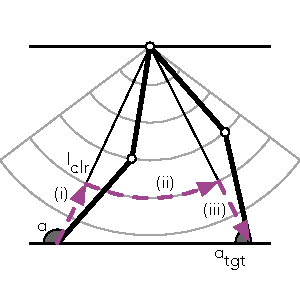
\includegraphics[width=\linewidth]{swing_leg_polar}
    \caption{The swing leg control guides the leg towards a desired landing leg
    angle $\alpha_\tn{tgt}$ through three phases: (i) Flex the knee until it
    achieves a clearance leg length $l_\tn{clr}$. (ii) Hold the leg length via
    knee damping. (iii) Stop and Extend the leg towards the ground when the leg
    reaches $\alpha_\tn{tgt}$. Figure reproduced from \citet{desai2012robust}.}
    \label{fig:swing_leg_polar}
\end{marginfigure}
\begin{align}
    \tau_\tn{k}^\tn{i} = \begin{cases}
                 0,                     & \dot{\alpha} > 0 \\
                -k^\tn{i} \dot{\alpha}, & \dot{\alpha} \le 0 
                \end{cases},
    \label{eq:flexphase}
\end{align}
where $k^\tn{i}$ is the flexion gain and the leg angle $\alpha$ is defined as
the angle between the horizontal and the hip-ankle line.  

The second phase activates when the leg length, defined as the distance between
the hip and ankle, contracts below a threshold. In this phase, the knee torque
is given by
\begin{align}
    \tau_\tn{k}^\tn{ii} = \begin{cases}
          -k_1^\tn{ii} \dot \phi_\tn{k}, & \dot \phi_\tn{k} \ge 0 \\
          -k_2^\tn{ii} \dot \phi_\tn{k}(\alpha - \alpha_\tn{tgt})
            (\dot{\alpha} - \dot \phi_\tn{k}), 
          & \dot\phi_\tn{k} < 0 \ \& \ \dot \phi_\tn{k} < \dot \alpha\\
          0, & \mathrm{otherwise}
      \end{cases},
    \label{eq:holdphase}
\end{align}
where $k_1^\tn{ii}$ and $k_2^\tn{ii}$ are damping coefficients. The first case
dampens knee flexion, while the second case dampens knee extension, but allows
progressively more extension as the leg angle approaches its target. The
modulation term $(\dot \alpha - \dot \phi_\tn{k})$ prevents premature landing of
the leg by damping the knee if it extends faster than the overall leg angle.

The third phase engages when the leg angle gets within a threshold of the
target leg angle. The control then applies torque to stop and extend the knee,  
\begin{align}
    \tau_k^\tn{iii} = 
    \begin{cases}
         k^\tn{iii}(\alpha_{\tn{thr}} - \alpha)
            \left(1 - \frac{\dot\alpha}{\dot\alpha_\tn{max}} \right), 
                & \alpha < \alpha_\tn{thr} \ \& \ \dot \alpha < \dot \alpha_\tn{max} \\
        0, & \tn{otherwise}
    \end{cases},
    \label{eq:stop}
\end{align}
where $\dot{\alpha}_{\mathrm{max}}$ is the maximum leg retraction velocity for
which the stopping knee torque is applied. When this torque brings the leg
velocity to zero, a knee extension torque is added,
\begin{align}
    \tau_\tn{k}^\tn{iii'} = \tau_\tn{k}^\tn{iii} - k^\tn{ext} (l_0 - l),
    \label{eq:extend}
\end{align}
where $l_0$ is the rest leg length, $l$ is the current leg length, and
$k^\tn{ext}$ is a proportional gain. 

The swing leg control also specifies a hip torque in the form of a proportional
derivative control on the leg angle, 
\begin{align}
    \tau_\tn{h}^\alpha = k_\tn{p} (\alpha - \alpha_\tn{tgt}) + k_\tn{d} \dot\alpha.
    \label{eq:hipfeedback}
\end{align}
This hip torque is supplemented by a feed forward term 
\begin{align}
    \tau_\tn{h} = \tau_\tn{h}^\alpha - 2 \tau_\tn{k}^\tn{iii}
    \label{eq:hipfeedforward}
\end{align} 
that neutralizes the coupling dynamics between the knee and hip during the
knee's stop and extend phase (Eq.~\ref{eq:stop}).

The torques produced by the swing controller augment the net torques produced by
the Hill-type muscles and reflexes during stance. At heel strike, the control
policy switches from using the swing leg control torques to the stance torques
generated by the muscle models. In late stance, the policy mixes the torques
specified by the stance and swing controllers by scaling the stance and swing
torques and muscle stimulations in proportion to the normalized ground reaction
force,
\begin{align}
    \tau_\tn{late stance} &= \tau_\tn{stance}(GRF) +
    \tau_\tn{swing}(1 - GRF),\\ 
    S^\tn{m}_\textrm{late stance}  &= S^\tn{m}(GRF).
\end{align}
During swing, only the swing leg torques are used.

\subsection{Neuromuscular Reflex Swing Leg Control}\label{sec:neuro_muscle_swing}
\begin{marginfigure}
    \centering
    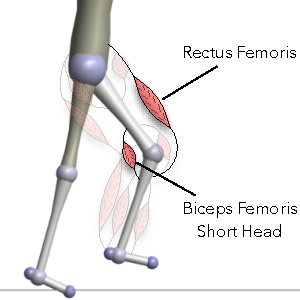
\includegraphics[width=\linewidth]{biped_w_muscles_rf_bfsh}
    \caption{Neuromuscular Swing leg control employs the seven muscles used in
    the stance control as well as a monoarticular knee flexor, the biceps
    femoris short head, and a biarticular hip flexor/knee extensor, the rectus
    femoris} 
    \label{fig:biped_w_muscles_rf_bfsh}
\end{marginfigure} 

The muscle reflex interpretation of the idealized swing leg control presented in
the previous \crefname{sec:neuro_ideal_swing} proposes reflexes to achieve the 
same three goals as the ideal swing leg control: (i) flex the knee to achieve
sufficient ground clearance, (ii) prevent toe scuffing by damping the knee (iii)
stop and extend the leg when the target leg angle is achieved (see
\cref{fig:swing_leg_polar}). This control assumes a leg with nine-muscles, the
seven included in the stance control (\cref{fig:biped_w_muscles}), as well as
two additional muscles shown in figure (\cref{fig:biped_w_muscles_rf_bfsh}).
These muscles are a monoarticular knee flexor, the biceps femoris short head,
and a biarticular hip flexor/knee extensor, the rectus femoris. As in the case
of the stance control, the reflexes primarily consist of linear feedback laws of
the form
\begin{align}
    \func{S}[phase][m]{t} = G_n^m \func{Pro}[n][]{t - \Delta t_n}.
\end{align}
For the swing control, the proprioceptive feedback can be either on length,
$\func{L}[n][m]{\cdot} = \func{l}[\tn{CE},n][]{\cdot} - l_{\tn{off}, n}$,
or velocity, $\func{V}[n][m]{\cdot} = \func{v}[\tn{CE},n][]{\cdot} -
v_{\tn{off}, n}$. In these equations $l_{\tn{off},n}$ and $v_{\tn{off}, n}$ are
offset lengths and velocities the control tries to obtain.

As in the idealized control, the knee control is divided into three phases. In
phase 1, the behavior of the idealized control is to provide knee flexion torque
in proportion to the rate of forward leg angle progression
(\cref{eq:flexphase}). The muscle interpretation uses the rate of length change
of the rectus femoris contractile element as a proxy for the speed of the leg
angle. It therefore implements phase 1 by stimulating a monoarticular knee
flexor, the biceps femoris short head, based on velocity feedback from the
rectus femoris.
\begin{align}
    \func{S}[i][\tn{bfsh}]{t} = G_\tn{rf}^\tn{bfsh}\func{V}[\tn{rf}][]{t_\tn{m}}.
\end{align}

In the second phase, the control dampens knee flexion and modulates the damping
of knee extension (\cref{eq:holdphase}, allowing more extension as the target
angle is approached and only damping the knee if it extends faster than the leg
angle progresses. In this phase, the control uses velocity feedback to dampen
knee flexion according to
\begin{align}
    \func{S}[\tn{ii}][\tn{rf}]{t} = G_\tn{bfsh}^\tn{bfsh}
        \func{V}[\tn{bfsh}][]{t_\tn{m}},
\end{align}
and a modified velocity feedback to dampen knee extension according to
\begin{align}
    \func{S}[\tn{ii}][\tn{bfsh}]{t} = G_\tn{bfsh}^\tn{bfsh}
        \func{V}[\tn{bfsh}]{t_\tn{m}} \func{L}[\tn{rf}][\tn{bfsh}]{t_\tn{m}} 
        \left( \func{V}[\tn{bfsh}]{t_\tn{m}} + \func{V}[\tn{rf}]{t_\tn{m}}
        \right).
\end{align}

The final task of the swing control, is to stop and extend the leg. Stopping is
achieved by length feedback on the hamstring
\begin{align}
    \func{S}[\tn{iii}][\tn{ham}]{t} = G_\tn{ham}^\tn{ham}
        \func{L}[\tn{ham}]{t_\tn{s}},
\end{align}
and is augmented by the other knee flexors if $\func{S}[\tn{iii}][\tn{ham}]{t} >
S_\tn{thr}$, where $S_\tn{thr}$ is a threshold.
\begin{align}
    \func{S}[\tn{iii}][\tn{bfsh}]{t} &= G_\tn{bfsh}^\tn{ham}
        \left (\func{S}[\tn{iii}][\tn{ham}]{t} - S_\tn{thr} \right) \\
    \func{S}[\tn{iii}][\tn{gas}]{t} &= G_\tn{gas}^\tn{ham}
        \left (\func{S}[\tn{iii}][\tn{ham}]{t} - S_\tn{thr} \right)
\end{align}
The control triggers knee extension through vastus length feedback, when the leg angle velocity crosses zero,
\begin{align}
    \func{S}[\tn{iii}][\tn{vas}]{t} = G_\tn{vas}^\tn{vas}
        \func{L}[\tn{vas}]{t_\tn{s}}.
\end{align}

The hip and ankle joints are controlled via length feedbacks. The hip control
approximates $\alpha$ through the length of the rectus femoris. Consequently,
the hip control uses length feedback from the rectus femoris in order to drive
the leg towards $\alpha_\tn{tgt}$,
\begin{align}
    \func{S}[][\tn{hfl}]{t} = S_0^\tn{hfl} + G_\tn{rf}^\tn{hfl}
        \func{L}[\tn{rf}]{t_\tn{s}} \\
    \func{S}[][\tn{glu}]{t} = S_0^\tn{glu} + G_\tn{rf}^\tn{glu}
        \func{L}[\tn{rf}]{t_\tn{s}}.
\end{align}
During swing length feedback on the tibialis anterior dorsiflexes the ankle to
prevent toe scuffing
\begin{align}
    \func{S}[][\tn{ta}]{t} = S_0^\tn{ta} + G_\tn{ta}^\tn{ta}
        \func{L}[\tn{ta}]{t_\tn{l}}
\end{align}
